\begin{figure}[tbp]
  \centering
  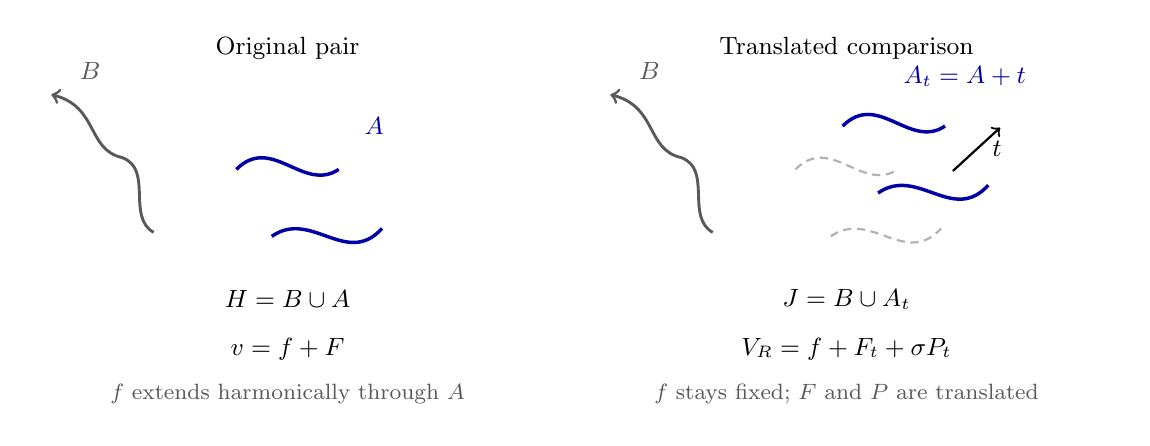
\begin{tikzpicture}[x=1cm,y=1cm,
      every node/.style={font=\small},
      fixed/.style={draw=black!65,line width=1.05pt},
      moving/.style={draw=blue!65!black,line width=1.25pt},
      old/.style={draw=black!30,line width=.8pt,densely dashed}]
    \path[use as bounding box] (-.05,-1.35) rectangle (13.85,3.6);

    \begin{scope}
      \node[anchor=north] at (3.25,3.6) {Original pair};
      \draw[fixed,<-] (.25,2.75)
        .. controls (.85,2.6) and (.7,2.05) .. (1.15,1.95)
        .. controls (1.55,1.8) and (1.2,1.2) .. (1.55,1.0);
      \node[anchor=east,text=black!65] at (1.0,3.05) {$B$};
      \draw[moving] (2.6,1.8)
        .. controls (3.05,2.25) and (3.45,1.5) .. (3.9,1.8);
      \draw[moving] (3.05,.95)
        .. controls (3.55,1.3) and (4.0,.55) .. (4.45,1.05);
      \node[text=blue!65!black] at (4.35,2.35) {$A$};
      \node at (3.25,.15) {$H=B\cup A$};
      \node at (3.25,-.48) {$v=f+F$};
      \node[font=\footnotesize,text=black!65] at (3.25,-1.05)
        {$f$ extends harmonically through $A$};
    \end{scope}

    \begin{scope}[xshift=7.1cm]
      \node[anchor=north] at (3.25,3.6) {Translated comparison};
      \draw[fixed,<-] (.25,2.75)
        .. controls (.85,2.6) and (.7,2.05) .. (1.15,1.95)
        .. controls (1.55,1.8) and (1.2,1.2) .. (1.55,1.0);
      \node[anchor=east,text=black!65] at (1.0,3.05) {$B$};
      \draw[old] (2.6,1.8)
        .. controls (3.05,2.25) and (3.45,1.5) .. (3.9,1.8);
      \draw[old] (3.05,.95)
        .. controls (3.55,1.3) and (4.0,.55) .. (4.45,1.05);
      \begin{scope}[shift={(.6,.55)}]
        \draw[moving] (2.6,1.8)
          .. controls (3.05,2.25) and (3.45,1.5) .. (3.9,1.8);
        \draw[moving] (3.05,.95)
          .. controls (3.55,1.3) and (4.0,.55) .. (4.45,1.05);
      \end{scope}
      \draw[->,line width=.8pt] (4.6,1.78) -- (5.2,2.33)
        node[midway,right=2pt] {$t$};
      \node[text=blue!65!black] at (4.75,2.98) {$A_t=A+t$};
      \node at (3.25,.15) {$J=B\cup A_t$};
      \node at (3.25,-.48) {$V_R=f+F_t+\sigma P_t$};
      \node[font=\footnotesize,text=black!65] at (3.25,-1.05)
        {$f$ stays fixed; $F$ and $P$ are translated};
    \end{scope}
  \end{tikzpicture}
  \caption{The comparison associated with a hypothetical separated compact
  piece $A$.  The remainder $B$ is fixed, while $A$ is translated by a small
  vector $t$ with $A_t\cap B=\varnothing$; the dashed curves mark its former
  position.  The displayed formula for $V_R$ holds in the inner comparison
  disk.  Far away, a cutoff returns the function to $v$.  The drawings are
  schematic: $A$ may contain several components, and no regularity of all of
  $A$ or $B$ is asserted.  The functions $F$ and $P$ need not have compact
  support.}
  \label{fig:compact-translation}
\end{figure}
